%%
%%	This is file 'Steine.tex'
%%
%%	This file is a sample LaTeX beamer presentation in German language which
%%	is considered to show you how themes look on your presentation.
%%	
%%	If the font size is too big for the theme, change it in line 28.
%%	The presentation theme can be changed in line 43.
%%
%%	IMPORTANT:
%%	The "Institut für artgerechte Haltung von Steinen, Gräfenberg" (line 48)
%%	is fictional and therefore not existing in reality.
%%
%%	---------------------------------------------------------------------------
%%	Copyright 2017 A. Arzberger and S. Friedl
%% 
%%	This work is licensed under a Creative Commons Attribution-ShareAlike 4.0
%%	International License (https://creativecommons.org/licenses/by-sa/4.0/).
%%
%%	This means that if you change the file and re-distribute it, you must re-
%%	tain the copyright notice header and license it under the same CC-BY-SA
%%	license.
%%
%%	---------------------------------------------------------------------------



\documentclass[11pt]{beamer}

\usepackage[utf8]{inputenc}
\usepackage[T1]{fontenc}

\usepackage{appendixnumberbeamer}
\usepackage{csquotes}
\usepackage{hyperref}

\usepackage[german]{babel}

\usepackage[osf,scale=.92]{roboto}
\usepackage[osf,slantedGreek]{mathpazo}

% CHANGE THE THEME USED FOR THE PRESENTATION HERE:
\usetheme{default}

\title{Steine}
\subtitle{Ein ernstzunehmendes Thema ...}
\author{A.~Arzberger \and S.~Friedl}
\institute[IaHS]{Institut für artgerechte Haltung von Steinen, Gräfenberg}

\begin{document}
	\frame{\maketitle}
	
	
	\section{Problemabgrenzung}
	\begin{frame}{Problemabgrenzung}
		\enquote{Steine sind aus unserem Alltag nicht wegzudenken und trotzdem behandeln wir sie wie leblose Objekte} \\
		-- \textit{nach \textsc{Hauke}}\footnote{\url{https://www.youtube.com/watch?v=ZOt64TtATMM}}
	\end{frame}


	\section[Natürlicher Feind]{Der natürliche Feind der Steine}
	\begin{frame}{Der natürliche Feind der Steine}
		\underline{Problem}:\hspace{1em} \textbf{\textsc{Massensteinhaltung}}
		\begin{itemize}
			\item Ausnutzung durch den Menschen
			\item unmögliche Lebensbedingungen
			\item Leben ohne Licht
			\item schwere Verletzungen durch Stapeln (z.~B. Kratzer, Brüche)
		\end{itemize}
		
		\bigskip
		
		\textbf{Der Mensch tritt die Würde der Steine mit Füßen!!}
	\end{frame}


	\section[Charakteristika]{Charakteristika von Steinen}
	\begin{frame}{Charakteristika -- Übersicht}
		\begin{itemize}
			\item \textbf{Sandstein}
					\begin{itemize}
						\item Entstehung: gepresster Sand
						\item Verwendung:
								\begin{itemize}
									\item Historische Bauten
									\item Gartensteine
								\end{itemize}
						\item \textsc{Achtung:} \\
							  Sandsteine sind leicht verletzbar!
					\end{itemize}
			\item und viele weitere Steine ...
		\end{itemize}
	\end{frame}


	\section[Artgerechte Haltung]{Artgerechte Haltung von Steinen}
	\begin{frame}{Artgerechte Haltung von Steinen}
		\begin{block}{Vorgaben}
			Haltung an der frischen Luft in großen Abständen
		\end{block}
	
		\begin{exampleblock}{Umsetzung}
			Freie Wiesen anmieten
		\end{exampleblock}
	
		\begin{alertblock}{Warnung}
			Steine, die eine hohe Geschwindigkeit aufweisen, könnten gefährlich werden ...
		\end{alertblock}
	\end{frame}


	\section{Zusammenfassung}
	\begin{frame}{Zusammenfassung}
		\begin{enumerate}
			\item wehrlose Steine werden ausgenutzt!
					\begin{enumerate}
						\item als Dekoration
								\begin{enumerate}
									\item im Garten
									\item in Parks
									\item in Schmuck
								\end{enumerate}
						\item als Spielzeug in Sandkästen
						\item als Gewicht
					\end{enumerate}
			\item Steine müssen artgerecht gehalten werden!
		\end{enumerate}
	
		\bigskip
	
		\textbf{$\rightarrow$ Das Leben der Steine ist grausam!}
	\end{frame}

	
	
	\appendix
	\frame{\frametitle{$ $}\centering\Huge\textbf{\textsc{Anhang}}}
	\begin{frame}{Zufriedenheit der Steine}
		\centering
		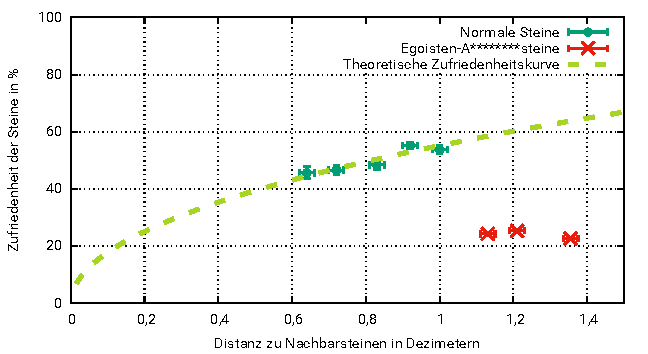
\includegraphics[width=.85\textheight]{zufriedenheit} \\
		
		\flushleft
		\textbf{\underline{\textsc{Merke:}}\hspace{1em} Steine sind Perfektionisten!}
	\end{frame}
\end{document}